\documentclass{article}
\usepackage[utf8]{inputenc}
\usepackage{hyperref}
\usepackage[T1]{fontenc}
\usepackage{lmodern}
\usepackage{layouts}
\usepackage[english]{babel}
\usepackage{microtype}
\usepackage{csquotes}

% Page layout
\usepackage{fancyhdr}
\usepackage[a4paper,width=150mm,top=30mm,bottom=30mm]{geometry}
\usepackage{multicol}
\setlength{\columnsep}{1cm}
\usepackage{changepage}

\pagestyle{fancy}
\fancyhf{}
\lhead{Marco Ballarin}
\rhead{\today}
\cfoot{Homework 1, Neural Network and Deep Learning 2020/21 \\  \thepage}
\renewcommand{\headrulewidth}{2pt}
\renewcommand{\footrulewidth}{1pt}

% Physics and math
\usepackage{physics}
\usepackage{amsmath}
\usepackage{amssymb}
\usepackage[sorting=none]{biblatex}
\addbibresource{bibliography.bib}

% Images
\usepackage{graphics}
\usepackage{pgfplots}
\pgfplotsset{compat=1.16}
\usepackage{xcolor}
\usepackage{subcaption}
\usepackage{float}
%\usepackage[cm]{fullpage}
\usepackage{gnuplottex}
\usepackage{mwe}

% Tables
\usepackage{booktabs} % Allow multicolumns in tables

% Code
\usepackage{listings}

\definecolor{codegreen}{rgb}{0,0.6,0}
\definecolor{codegray}{rgb}{0.5,0.5,0.5}
\definecolor{codepurple}{rgb}{0.58,0,0.82}
\definecolor{backcolour}{rgb}{0.95,0.95,0.92}

\lstdefinestyle{mystyle}{
    language=python,
    backgroundcolor=\color{backcolour},   
    commentstyle=\color{codegreen},
    keywordstyle=\color{magenta},
    numberstyle=\tiny\color{codegray},
    stringstyle=\color{codepurple},
    basicstyle=\ttfamily\footnotesize,
    breakatwhitespace=false,         
    breaklines=true,                 
    captionpos=b,                    
    keepspaces=true,                 
    numbers=left,                    
    numbersep=5pt,                  
    showspaces=false,                
    showstringspaces=false,
    showtabs=false,                  
    tabsize=2
}
\lstset{style=mystyle}

\newcommand{\tb}[1]{\textbf{#1}}


\begin{document}


% Title
\begin{center}
    \huge
    \textbf{Supervised Deep Learning}  % title
    
    \normalsize
    \vspace{0.4cm}
    \textbf{Marco Ballarin} 1228022  \\ % Author
    marco.ballarin.6@studenti.unipd.it

    \vspace{0.5cm}
    \Large
    \textsc{ Abstract}
    \begin{adjustwidth}{30pt}{30pt}
    \normalsize
    \vspace{0.3cm}
    In this report we will review several tasks related to unsupervised learning, focusing on the models called autoencoders.
We will optimize their architecture and employ them for different tasks, like image generation, denoising and transfer learning. We will 
finally implement a more advanced type of autoencoder, the Variational Autoencoder, and analyze its performances. We will use the
MNIST dataset.
    \end{adjustwidth}
\end{center}
\vspace{0.2cm}
%\maketitle
%\tableofcontents
%\begin{multicols}{2}

\section{Introduction \label{sec:int}}
In this report we will tackle two different problems using the supervised deep learning framework. This means that we will
have datasets $D$ formed of couples $\{(x_i,y_i)\}_{i=1,\dots,N}$, where $x_i$ are the samples and $y_i$ the labels.
The report will be divided into four main Sections:
\begin{enumerate}
    \item Introduction, where we introduce our work;
    \item Regression, where through a deep neural network we try to predict the behavior of a curve;
    \item Classification, where through a convolutional neural network we try to classify the handwritten digits from $0$ to $9$ using
        the MNSIT dataset;
    \item Appendix, where we will add images that are not fundamental for the flow of the report, but may be useful.
\end{enumerate}

\section{Regression \label{sec:reg}}

\subsection{Methods \label{sec:meth_reg}}
For the regression task it is better to use a reduced number of hidden layers, and in particular we choose to use $2$ of them.
Our network will so be composed of:
\begin{itemize}
    \item An input layer of one neuron;
    \item A first hidden layer oh $N_h$ neurons;
    \item A second hidden layer of $2\cdot N_h$ neurons;
    \item An output layer of one neuron.
\end{itemize}
To avoid vanishing problems in the gradient we will use a rectified linear unit (ReLU) as activation function.
This simple topology in the network is due to the fact that this problem is "simple" from the neural networks point of view, and adding too many parameters we 
will be easily led to overfitting. We will so make an extensive use of regularization procedures to avoid these problems. In 
particular, we will use two main methods:
\begin{enumerate}
    \item dropout, which consists of randomly eliminate neurons during the training with probability $p_{drop}$.    
    \item L2 regularization, which consists of adding a penalty in the loss proportional to the 2-norm
        of the parameters, i.e. weights and biases. We stress that in pytorch this method is enabled not in the loss
        function but in the optimizer, using the \lstinline{weight_decay} keyword.
\end{enumerate}
However, implementing both forms of regularizations generated sub-optimal results. We so decided to put to $0$ the L2
regularization, stressing that we can do this without losing generality.

We will try two different optimizers:
\begin{enumerate}
    \item The stochastic gradient descent with momentum, which is the really basic algorithm for optimization.
        The addition of the momentum, i.e. the memory of previous steps, really helps to go out of local minima and speeds up convergence;
    \item the Adam algorithm, adaptive moment estimator, a more advanced algorithm that uses estimations of first and second 
        moments  of the gradient to adapt the learning rate of each weight of the neural network.
\end{enumerate}
The amount of data available for this task is quite limited, we will so apply a cross-validation technique to perform the 
hyper parameters tuning. This method consists of splitting the training test into $k$ different folds and then, for each
hyper parameters set, train the network on the union of $k-1$ folds, performing the validation on the one which is missing.
This approach ensure also better performances, since the validation set is different for each of the iterations, and so we
cannot end up with a model that perfectly fits one given validation set.
After the hyper parameters choice is done, we will train the model over the full training test.

We will then optimize the number of hidden units in the layers of the network, the learning rate and the number of epochs
needed for the training procedure.

Lastly, we will visualize the network features: in particular we will plot the weights histograms and the activation profiles.
We will see that we can actually extract a lot of information, in particular from the activation profiles.

\subsection{Results \label{sec:res_reg}}
The best performing network is reported in Figure \ref{fig:reg_net}.
\begin{figure}[h]
    \centering
    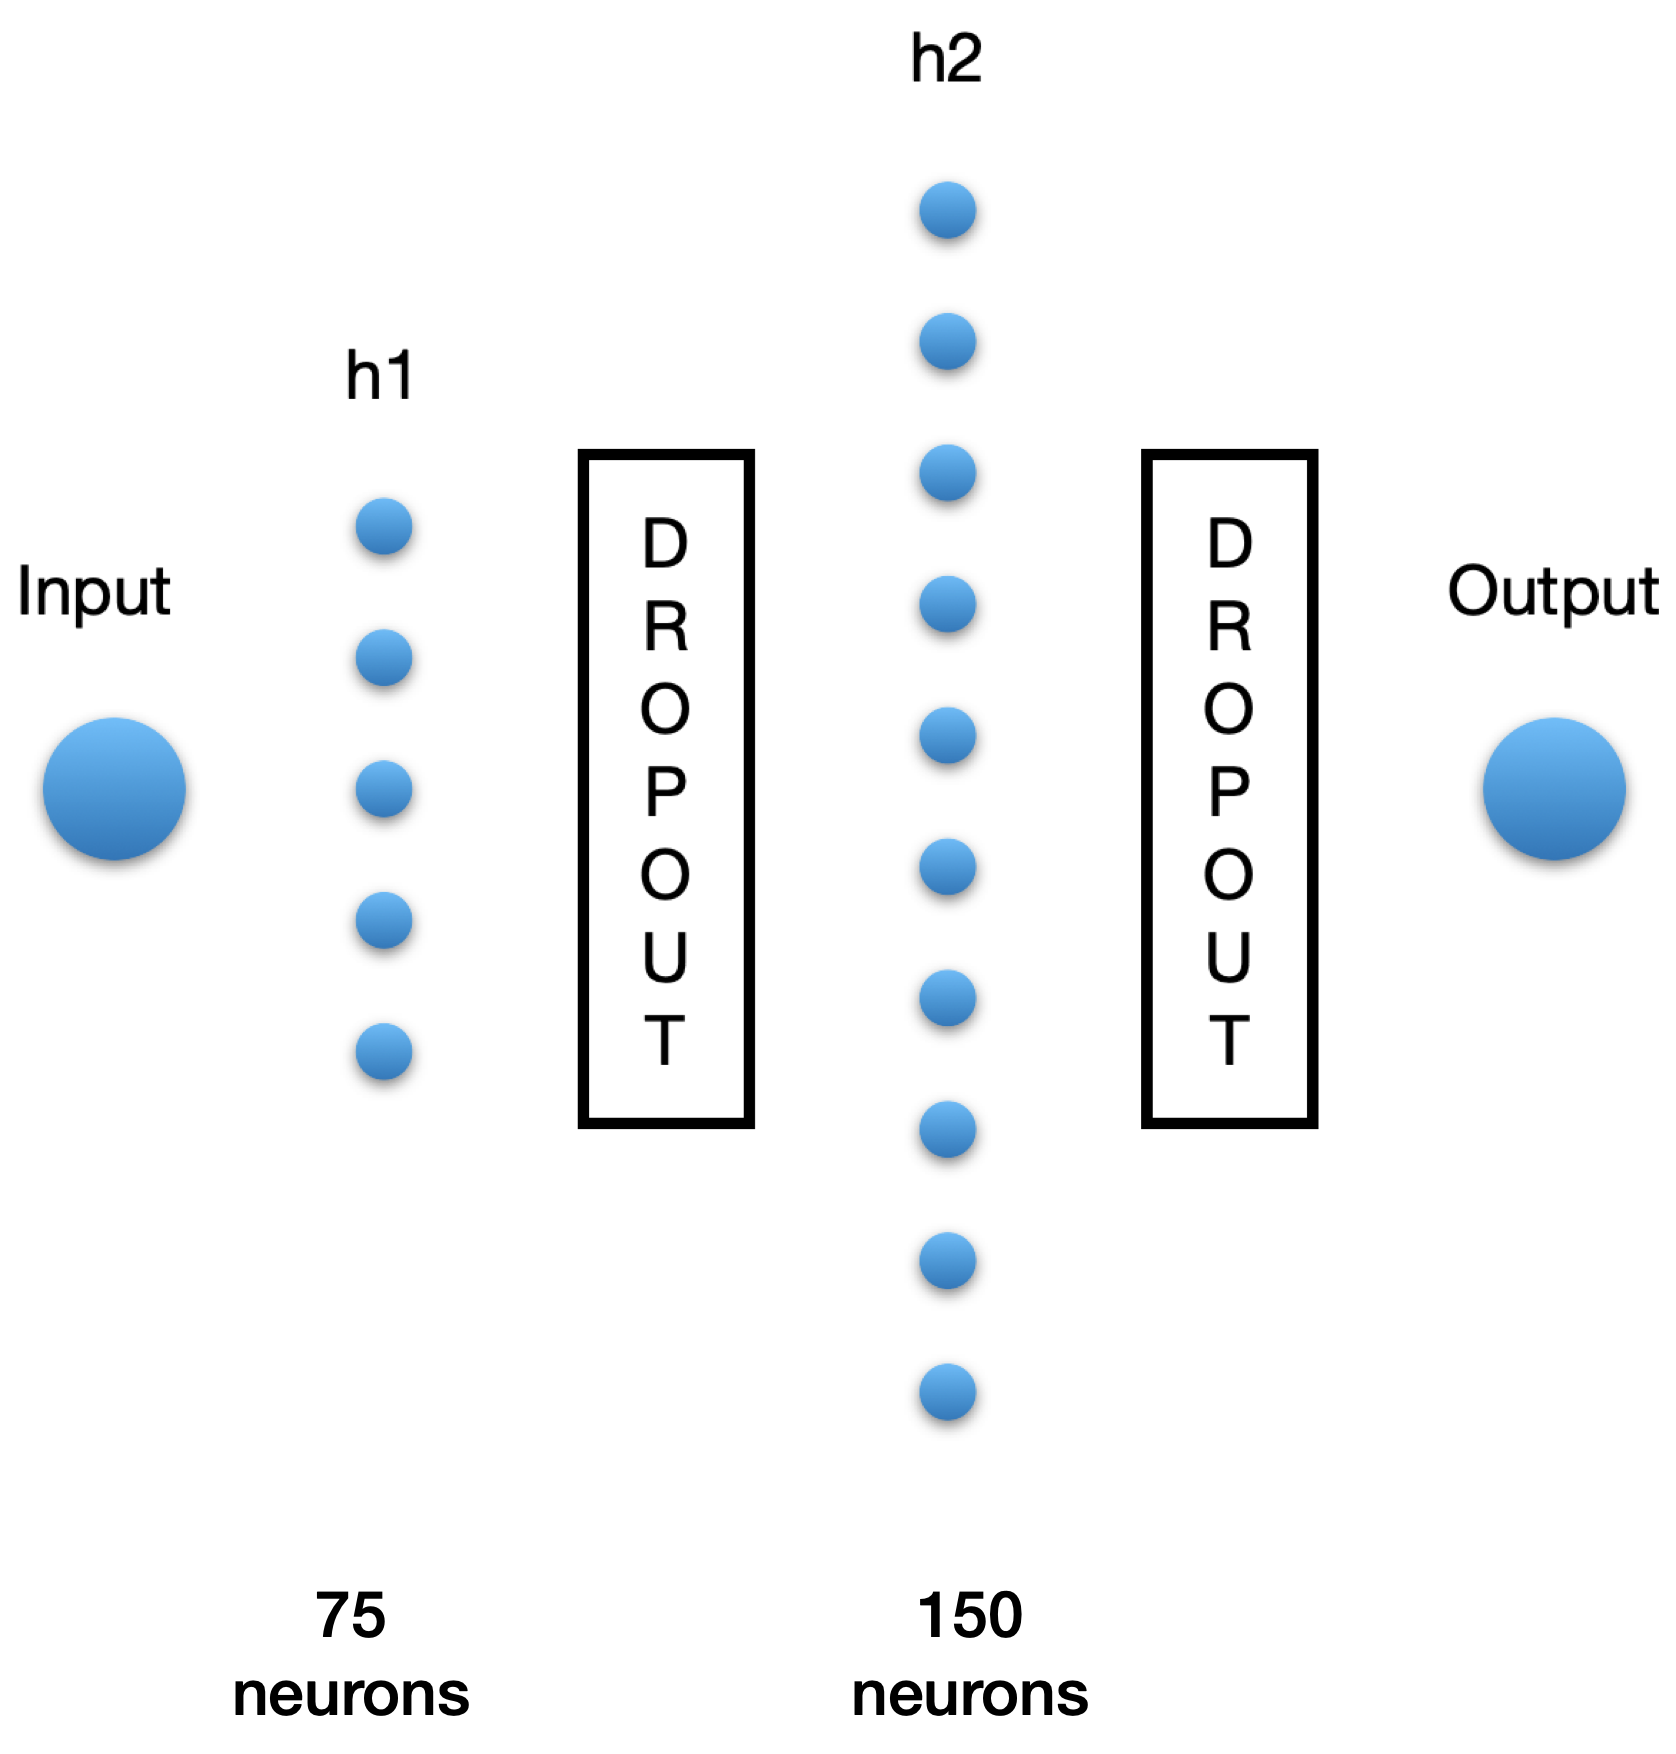
\includegraphics[width=0.5\textwidth]{Images/Regression_network.png}
    \caption{Final network for the regression task.}
    \label{fig:reg_net}
\end{figure}

\section{Classification \label{sec:class}}
\subsection{Methods \label{sec:meth_class}}
In the classification task we have to develop a network which classifies the MNIST dataset, i.e. the dataset containing handwritten
digits from $0$ to $9$. This dataset is quite exhaustive, and so we will not need to apply the Cross-validation technique.
The size of this dataset present nevertheless another challenge: the training time can become too long. For this reason we really
need to finely optimize the number of epochs we use in this procedure. One possible solution would be, as in the previous case,
use them as a hyper parameter. However, we will waste a lot of computational resources in this search. We so decided to apply
a technique that is called early stopping: if the validation loss $l_{v}$ does not diminish sufficiently in a given number of
epochs then we kill the training loop. In this way we can get rid of poorly initialized networks and have an overall speed up
of the process. In particular, calling $\vec{l}^{(t)}=(l_{v}^{(1)},l_{v}^{(2)}, \dots, l_{v}^{(t)} )$ the vector containing all the losses at iteration $t$, with a maximum number
of iteration $T$ we stop the process if:
\begin{equation}
    \bar{l} - l_v^{(t)} < 0.01 \hspace{0.5 cm} \mbox{with } \begin{cases}\bar{l}= \frac{1}{t-\tau}\sum_{i=\tau}^t l_v^{(i)} \\ \tau=\min(t, T/10)
    \end{cases}
\end{equation}

The other main difference with respect to the regression task is that the dataset is composed by images. For this reason we 
decided to use two convolutional layers at the beginning of the network. These layers make use of filters, i.e. feature maps
that are applied along all the image with the same weights. We will use filters of dimension $3\times3$. This means that we
will several small $3\times3$ feature maps that will enhance the same details along all the figure. The remarkable example 
in this framework are filters which enhance edges. We will analyze them in Section \ref{sec:res_class}.

Through a random search we will optimize the following parameters:
\begin{itemize}
    \item The dropout;
    \item The learning rate;
    \item The optimizer, choosing from stochastic gradient descent and Adam;
    \item the strength of the L2 regularization,
\end{itemize}

To further enhance the dataset we will apply a random rotation of $45°$ and some Gaussian noise. To help the network in the learning
phase we will also normalize the inputs, using the apposite pytorch transformation. We present the network structure in Figure \ref{fig:cl_net}
\begin{figure}[h]
    \centering
    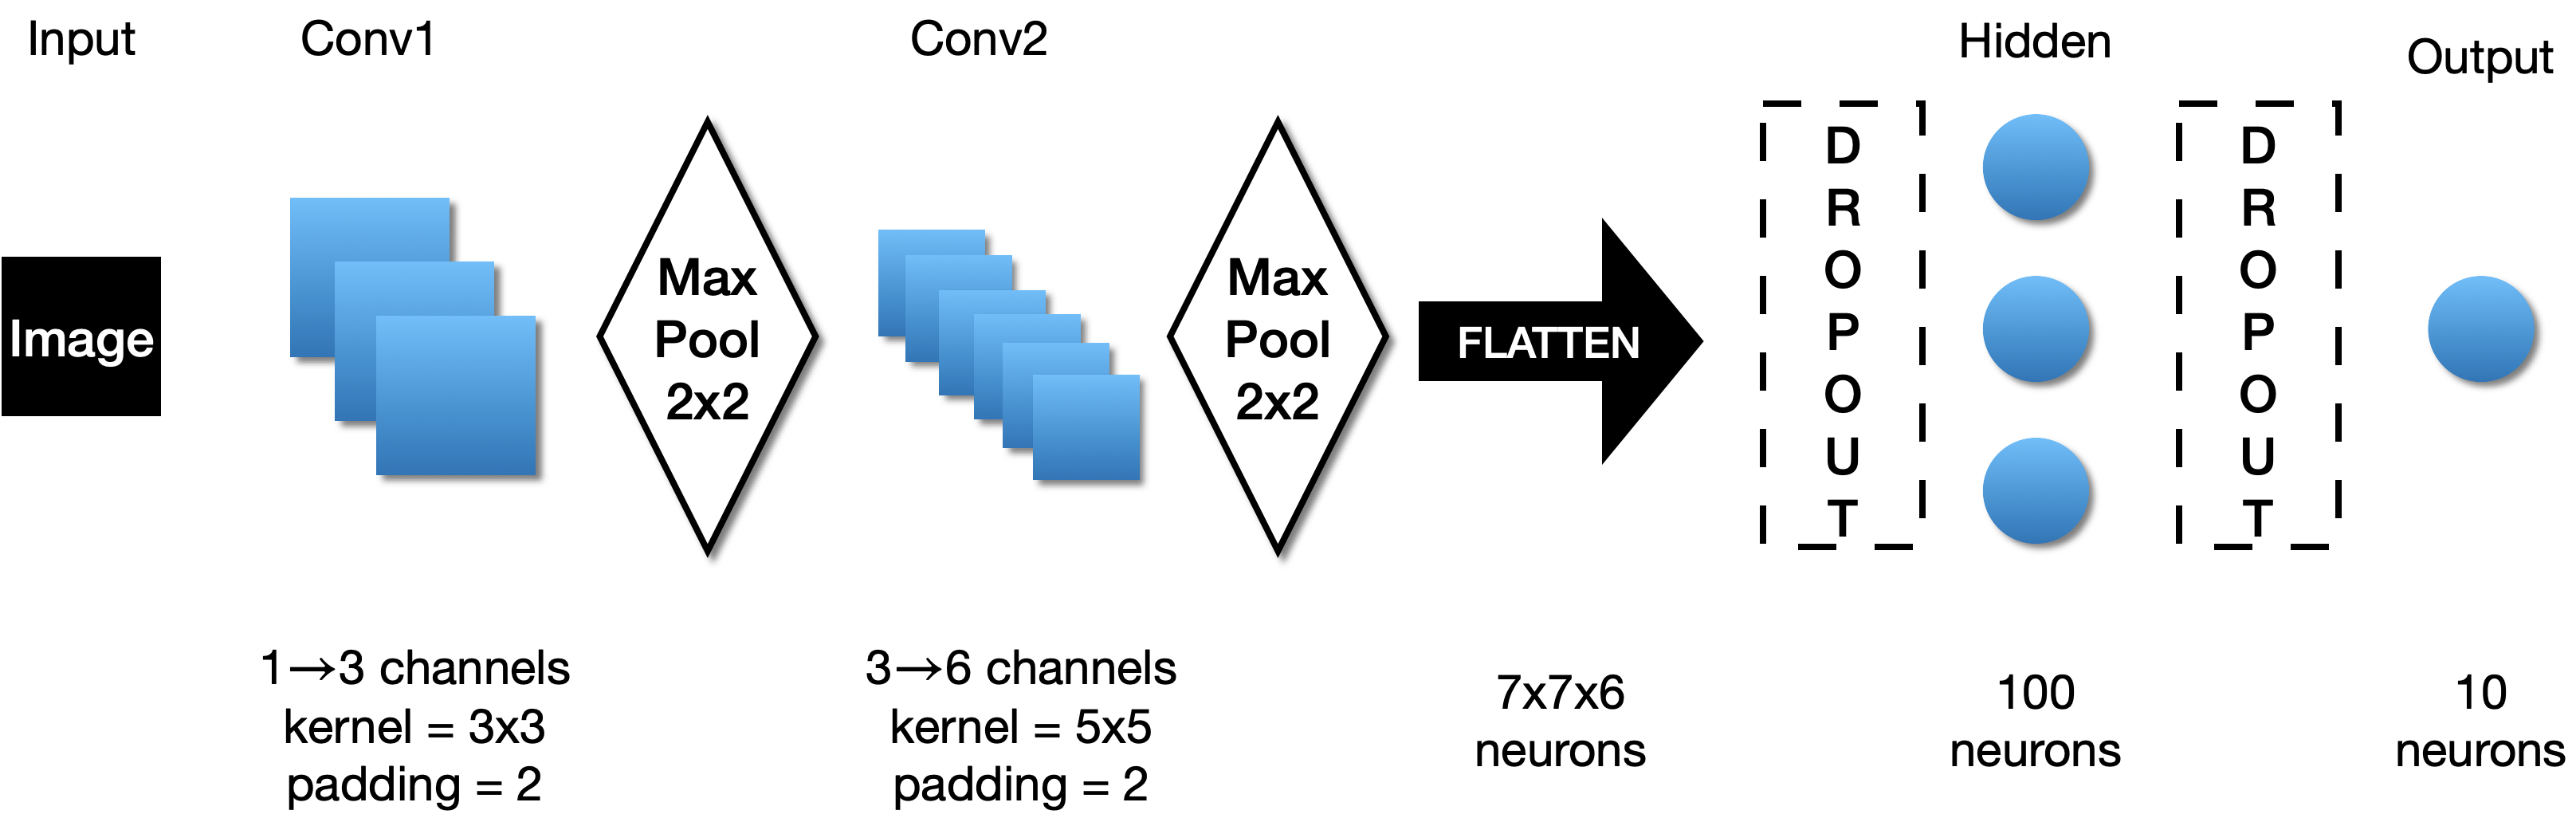
\includegraphics[width=0.8\textwidth]{Images/clas_net.png}
    \caption{Network structure for the classification task. The activation function used is the rectified linear unit.
    The output digit is selected as the argmax among the $10$ output neurons.}
    \label{fig:cl_net}
\end{figure}

\subsection{Results \label{sec:res_class}}
We present the grid search space in Figure \ref{fig:cl_hp}, and report the best parameters found in 
Table \ref{tab:cl_par}. With this set of parameter the network results fully trained in only $7$ epochs.
\begin{table}[h]
    \centering
    \begin{tabular}{cccc} \hline
        Dropout & Learning rate & Optimizer & Regularization  \\ \hline
        $0.1$   & $0.003$       & Adam      & $0.001$         
    \end{tabular}
    \caption{Optimal parameters for the classification task.}
    \label{tab:cl_par}
\end{table}
We can see that the regularization, through both the dropout and the L2 regularization, is higher in this case, meaning that this 
task requires particular attention to avoid overfitting.

The accuracy on the test set of the model gave optimal results, with an accuracy of $0.999$.

We present in Figure \ref{fig:cl_f1} the filters of the first convolutional layer and in 
Figure \ref{fig:cl_f2} the filters of the second convolutional layer. They are, however, of difficult interpretation. We can 
however see in Figure \ref{fig:cl_f2} a pattern that suggests that these filters are looking for edges in the figures.
\begin{figure}[h]
    \centering
    \begin{minipage}[t]{0.48\textwidth}
        \centering
        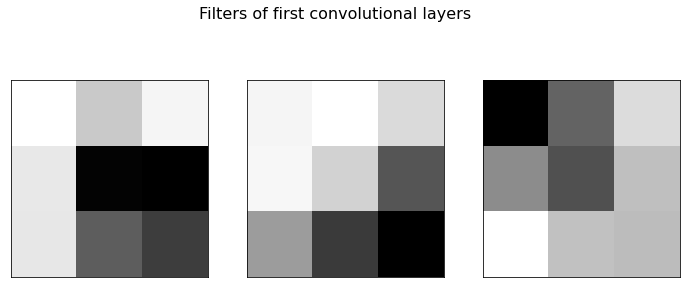
\includegraphics[width=0.98\textwidth]{Images/clas_filt1.png}
        \caption{$3\times3$ kernels of the filters of the first convolutional layer. It is not particularly clear which are
        the enhanced features. }
        \label{fig:cl_f1}
    \end{minipage}\hfill
    \begin{minipage}[t]{0.48\textwidth}
        \centering
        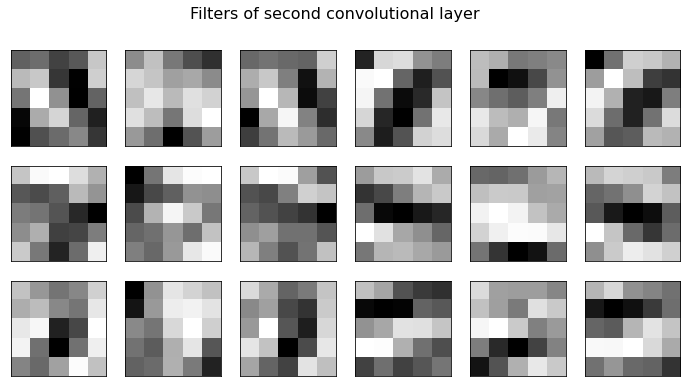
\includegraphics[width=0.98\textwidth]{Images/clas_filt2.png}
        \caption{$5\times5$ kernels of the filters of the second convolutional layer. We can observe black lines, which correspond
        to an enhancement of the edges.}
        \label{fig:cl_f2}
    \end{minipage}
\end{figure}

It is more interesting to analyze the activation profiles of the convolutional layers. In Figure \ref{fig:cl_a1} we can 
observe in a really clear way the digit that was given in input, while in \ref{fig:cl_a2} we can observe the enhancement 
of the edges of that number, as suggested by the filter.
\begin{figure}[h]
    \centering
    \begin{minipage}[t]{0.48\textwidth}
        \centering
        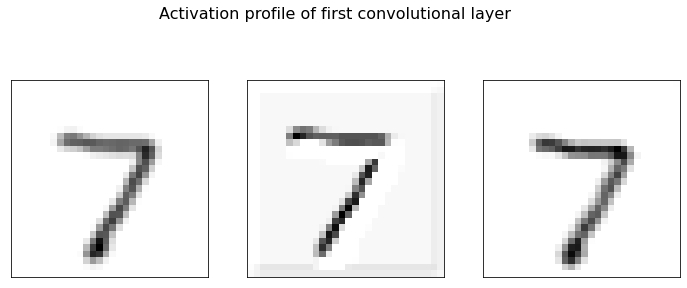
\includegraphics[width=0.98\textwidth]{Images/clas_act1.png}
        \caption{The three channels in output from the first convolutional layer. We can observe the input digit, which is a
        $7$. }
        \label{fig:cl_a1}
    \end{minipage}\hfill
    \begin{minipage}[t]{0.48\textwidth}
        \centering
        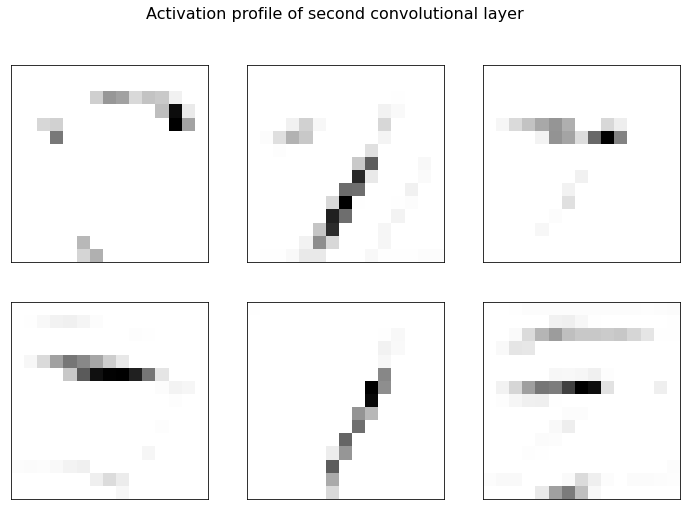
\includegraphics[width=0.98\textwidth]{Images/clas_act2.png}
        \caption{The six channels in output from the second convolutional layer. We can observe a decomposition of the input 
        digit in edges, which is common in convolutional networks. }
        \label{fig:cl_a2}
    \end{minipage}
\end{figure}

\section{Appendix \label{sec:app}}
We present here images that can be interesting but are not fundamental for the report.
\begin{figure}[h]
    \centering
    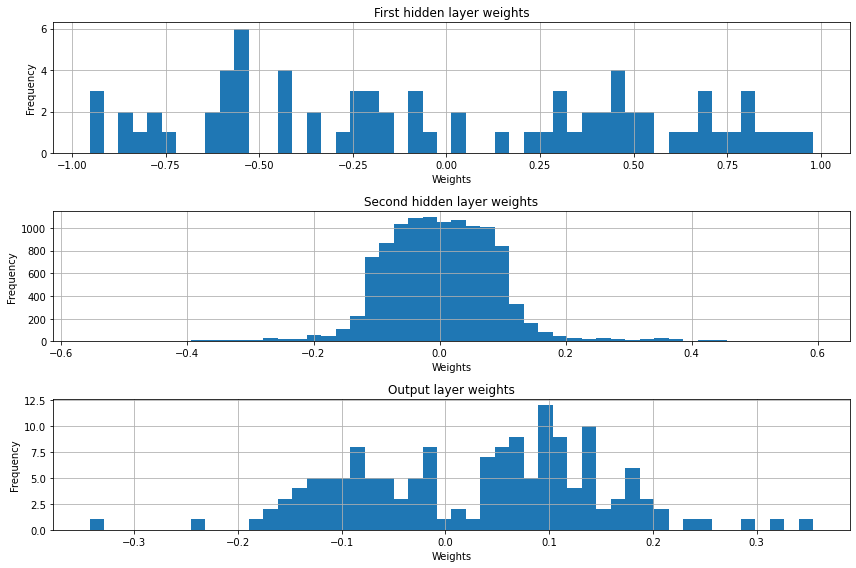
\includegraphics[width=0.8\textwidth]{Images/reg_weights.png}
    \caption{Weight histograms for the different layers of the network.}
    \label{fig:reg_weights}
\end{figure}

\begin{figure}[h]
    \centering
    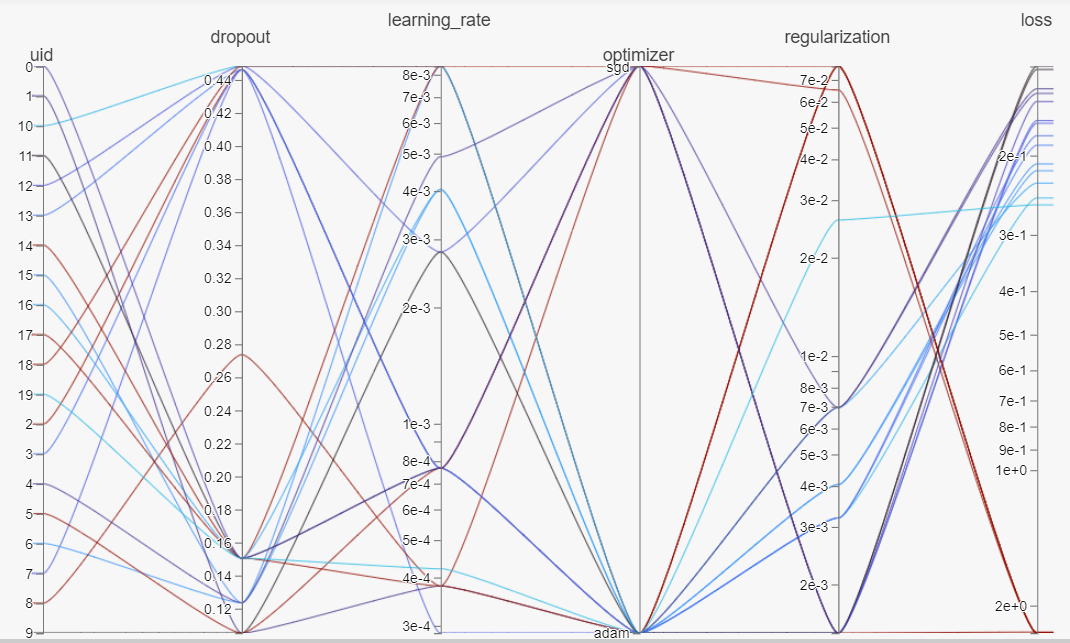
\includegraphics[width=0.8\textwidth]{Images/hyperparams.PNG}
    \caption{Hyperparameters search for the classification task. We plotted with a color which is proportional to the loss function,
    reported in log-scale. The darker the color, the better the result. We notice that a really high L2 regularization 
    usually translates in a low loss score.}
    \label{fig:cl_hp}
\end{figure}

%\end{multicols}

% Uncomment if you have a bibliography
%\printbibliography

\end{document}
